The following subsections will discuss what is necessary for communication in multiplayer games.
Human communication can roughly be divided into verbal communication and non-verbal communication \autocite{Kujanpaa2003SupportingAvatars}[2]. 
Apart from that, the reason why common ground is needed for players will be treated. Also the embodiment of players within virtual worlds and the collaborative virtual environment will be described.



\subsection{Verbal Communication}
\label{section:Verbal Communication}

People use voice or text for communication, which is known as verbal communication.
Voice however cannot only be used to spread information.
For evolutionary reasons, humans have come to use voice to determine gender, personality, intentions etc. \autocite{Williams2007CanCommunity}[427].

Most Massive multiplayer online games were using text-based chat systems.
\textcite{Williams2007CanCommunity} say that although text communication lacks vocal and expression-based cues, it provided different kinds of people to connect and interact with each other. As they are unable to see one another and likely less aware of their differences, conversations can be about their mutual interests or activities, being less hampered by restrictive social norms based purely on their demographics \autocite{Williams2007CanCommunity}[428].

With telecommunication and the internet, communication over large distance became possible. Before Voice over IP (VoIP) was invented, players were only able to communicated with each other text based. Voice chat may, when compared to text, improve the bridging function through the expansion of social cues, bringing communication closer to the presumed gold standard of face to face communication \autocite{Williams2007CanCommunity}[431].

Players use verbal communication in games to maintain mutual understanding, form strategies and share experiences as well as their current game status \autocite{Cheung2012CommunicationGaming}[572].

In fast paced FPS-games, players use callouts for very fast sharing of information. \textcite{Tang2012VerbalGames}[581] found during a study, that these callouts are often eight words or fewer. As a response, players will get short answers as feedback.
However, to understand such short phrases, players have to understand the game environment and game mechanics, so they can predict the teammate to understand everything in an appropriate way \autocite{Tang2012VerbalGames}. This is connected to the term common ground in section \ref{section:Common Ground}. Players always have to know the structure of the game, so they can talk about it without too many misunderstandings.

The ability of voice communication is also positively affecting the player performance. \textcite{Vaddi2016Investigating2}[46] showed during a test, that players who can use voice and in-game communication mechanics had the best performance, followed by voice only communication. Potentially as players become more comfortable with the game and its mechanics, the communication mechanics matter even less \autocite{Vaddi2016Investigating2}[46]. Therefore, the verbal communication seem to have an even bigger impact on advanced players.




\subsection{Nonverbal Communication}
\label{section:Nonverbal Communication}

\begin{figure}
    \centering
    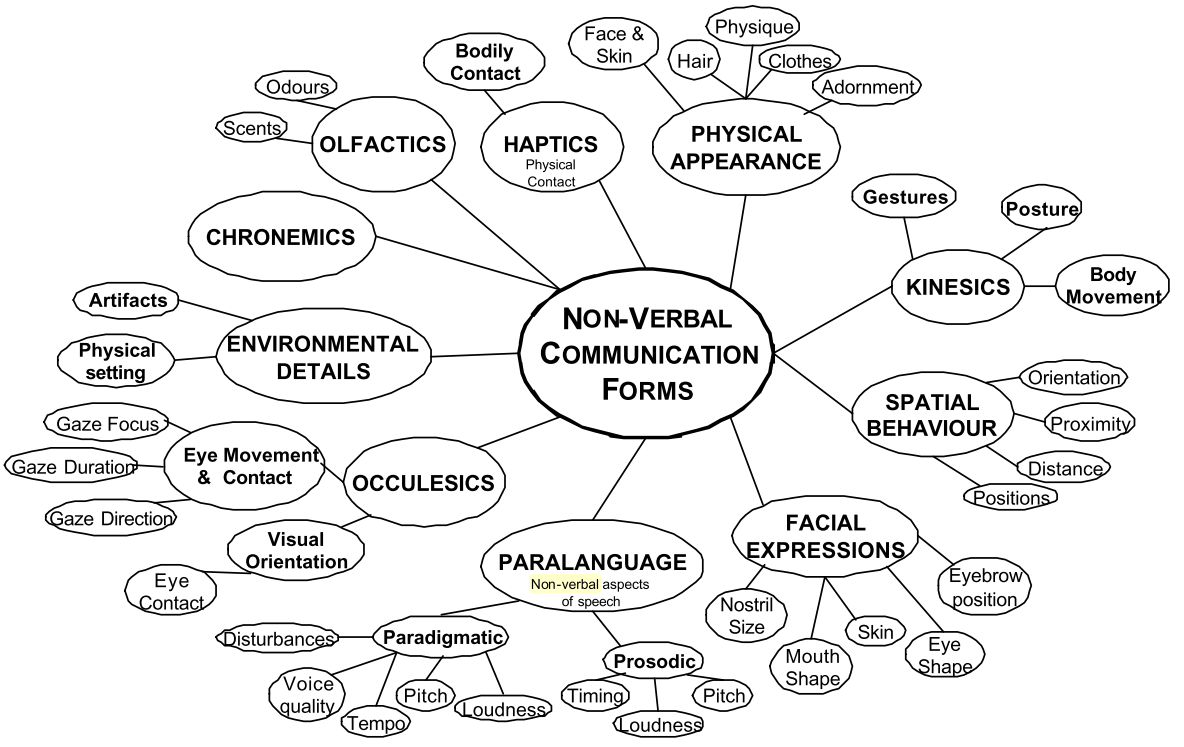
\includegraphics[width=0.95\textwidth]{images/non-verbal_communication_forms.png}
    \caption{ Concept model depicting the non-verbal communication forms
    \break
    \autocite{Manninen2002PlayerSession}[7]. }
    \label{fig:non-verbal communication forms}
\end{figure}

People use non-verbal communication to coordinate actions in all aspects of daily life, including the use of body movements, pointing, touching, gazing, and so on \autocite{Leavitt2016PingGames}[4338].

During fast gameplay in co-located games, \textcite{Cheung2012CommunicationGaming}[576] observed nearly no non-verbal communication, concerning face to face communication.
Looking away would introduce too high risk of awareness or communication breakdowns and removing the hands of the controller could have dire consequences during playing \autocite{Cheung2012CommunicationGaming}[576]. Anyway, this physical based non-verbal communication is only feasible during co-located multiplayer games.


In figure \ref{fig:non-verbal communication forms}, many different forms of non-verbal communication forms are displayed. A lot of them can be transferred from physical to virtual space. The visual elements, physical appearance, kinetics and facial expressions can be used to support the design of more communicative computer game avatars \autocite{Kujanpaa2003SupportingAvatars}[6].

Computer games can also have additional non-verbal communication elements, which are not always possible in the physical world. As example, players in Portal 2 can coordinate their actions using ping tools \autocite{Vaddi2015Validating2}[722]. With free hand annotations in Dota 2, players can create a drawing on the minimap \autocite{Wuertz2017Why2}[1979].


\subsubsection{Gestures}

Physical gestures are limited to co-located multiplayer games and players are also often hindered of using them, as removing the hands from the game controller may have negative consequences \autocite{Cheung2012CommunicationGaming}[570]. Besides physical gestures, virtual environments enable players to use virtual gestures as well.

Virtual gestures are gestures within the game, used by an avatar to indicate objects, areas and directions \autocite{Cheung2012CommunicationGaming}[573].
Also pointing with a weapon or shooting at ammunition instead of describing its location is a common scenario \autocite{Cheung2012CommunicationGaming}[573]. Some gestures seem to be already understood by players from their previous gaming experiences, as they do not explain or discuss some virtual gestures \autocite{Cheung2012CommunicationGaming}[574].

\textcite{Wuertz2017Why2} observed during two studies why gestures were created and found six distinct motivations: planning, warning, resource, conflict, help, and emotion.
Therefore, virtual gestures and other virtual non-verbal communication forms can be expanded by implementing mechanics, which enable collaboration. In Section \ref{Cooperative game mechanics}, such cooperative game mechanics will be discussed further.

\subsection{Common Ground}
\label{section:Common Ground}

When two people talk with each other, they will assume knowledge about certain things, which means the other one has to be aware of the background information the discussion is about. The example of \textcite{Stalnaker2002CommonGround}[702] is the sentence "The king of France is bald", that presupposes that France has a unique king. This stack of information is called common ground. 

A representation of the common ground helps to clarify both of the ends of the communicative action by representing the possibilities among which the speaker intends to distinguish, and the means available to the speaker to distinguish between them - the information that must be available in order for the act of uttering certain noises reasonably be taken as an act of trying to get someone to acquire certain information \autocite{Stalnaker2002CommonGround}[702].
If a presumption is not known at a certain point, it will come to existence at this certain point, which is called the phenomenon of \textit{presupposition accommodation} \autocite{Stalnaker2002CommonGround}[705].

The start point of the common ground during a conversation can be a common or mutual belief, something everybody knows and everybody knows that the knowledge is also present for everybody else. However, there can be false assumptions, that other people know it as well, which then cannot be counted to common belief.
Since common beliefs and beliefs about common beliefs are derivative from individual beliefs, the way they change in the course of a conversation will be determined by ordinary belief changes \autocite{Stalnaker2002CommonGround}[708].
Therefore, the common belief is not static during a conversion and both types of beliefs will change during the ongoing conversation. This process by which something becomes common ground in virtue of one party recognising that the other takes it to be common ground, is called accommodation \autocite{Stalnaker2002CommonGround}[712]. 
Assumptions one person makes can become part of the common ground of the discussion if it is accepted by others, even if it is only temporary.


\textcite{Clark2004GroundingCommunication.}[222] said that it takes two people to work together for certain things and both have to coordinate the content and process of what they are doing to succeed in it.
In other words, common ground is the basis a conversation needs to be successful. Information is pre-assumed and can differ from others. If that happens, the group has to agree on what they are talking about.  


\subsection{Embodied Communication}
\label{section:Embodied Communication}

Embodying communication entails that the individuals engaged in communication have a body with which they are presented in the world, and that they can only communicate through this body, as opposed to through some kind of direct or indirect way to transfer meaning \autocite{Galantucci2012TheHumans}[229].

This embodiment implies, that partners which can communicate have limited knowledge of what each of them perceives or knows \autocite{Galantucci2012TheHumans}. Therefore, telepathy and automatic shared information is not part of it. Additionally, every player needs to have a different perspective to gather information separately from each other, which can then be shared by communicating. 

According to \textcite{Vaddi2016Investigating2}, a player avatar, which is capable of communication through cooperative communication mechanics, offers players a means to communicate in an embodied way.

The player avatar can be seen as a representation of the other player. Thus, teammates will know where the player is currently positioned, where the player is going to, may see what someone is planning, and so on.


\subsection{Collaborative Virtual Environments}
\label{section:Collaborative Virtual Environments}

Collaborative virtual environments (CVE) are virtual worlds shared by participants across a computer network \autocite{Benford2001CollaborativeEnvironments}[79]. In computer games, players are provided a player avatar, which enables players to communicate in a embodied way, described before (Section \ref{section:Embodied Communication}). The game-world itself is a collaborative virtual environment. Players are able to interact with each other, as long as they are part of the same environment.

Players in online multiplayer games are rarely physically side by side. During studies of cooperative work, real-world environment have highlighted the important role of physical space as a resource for negotiating social interaction \autocite{Benford2001CollaborativeEnvironments}[80]. Therefore, CVEs have the potential to take the same part as physical space in virtual communication platforms.
Within this CVEs, avatars present their identity, presence, location and activities, which can be graphically seen by others \autocite{Benford2001CollaborativeEnvironments}[79].
Furthermore \textcite{Maher2011DesignersEnvironments}[3] notes in her work that communication among the participants in a CVE is often about location and viewpoints, allowing individuals to pursue their own tasks as well as have their attention focused on a shared task.